\documentclass[border=3pt]{standalone}
% Shared preamble of the block diagrams: LaTeX fonts (Latin Modern, as in the thesis text) and TikZ styles.
% Compile with build.sh (needs pdflatex + TikZ). In the thesis, just include the compiled PDFs.
\usepackage[T1]{fontenc}
\usepackage{lmodern}
\usepackage{amsmath,amssymb,bm}
\usepackage{tikz}
\usetikzlibrary{arrows.meta,calc,fit,backgrounds}

\definecolor{boxblue}{RGB}{218,232,245}   \definecolor{edgeblue}{RGB}{143,180,220}
\definecolor{boxgreen}{RGB}{226,240,217}  \definecolor{edgegreen}{RGB}{140,190,120}
\definecolor{boxteal}{RGB}{213,238,240}   \definecolor{edgeteal}{RGB}{110,190,196}
\definecolor{boxpurple}{RGB}{232,224,243} \definecolor{edgepurple}{RGB}{170,140,205}
\definecolor{boxorange}{RGB}{252,228,214} \definecolor{edgeorange}{RGB}{240,160,115}
\definecolor{fwdc}{RGB}{62,106,153}       \definecolor{invc}{RGB}{232,98,44}
\definecolor{navy}{RGB}{31,58,95}         \definecolor{muted}{RGB}{90,100,115}

\tikzset{
  >=Stealth,
  icon/.style  ={draw=edgeblue, fill=boxblue, rounded corners=3pt, line width=0.6pt, minimum width=1.5cm, minimum height=1.15cm},
  block/.style ={draw=edgeblue, fill=boxblue, rounded corners=3pt, line width=0.6pt, align=center, text=navy, inner sep=4pt, font=\small},
  plain/.style ={draw=black, fill=white, rounded corners=3pt, line width=0.8pt, align=center, inner sep=4pt, font=\small},
  fwd/.style   ={-{Stealth[length=5pt,width=4pt]}, line width=0.9pt, color=fwdc},
  inv/.style   ={-{Stealth[length=5pt,width=4pt]}, line width=0.9pt, color=invc, dash pattern=on 3pt off 2pt},
  group/.style ={rounded corners=4pt, line width=0.9pt, dash pattern=on 4pt off 3pt},
  note/.style  ={font=\footnotesize, text=muted, align=center},
}
% plate icon: rectangle with resonator dots; #1 centre, #2 dots "x/y, x/y" in [-1,1]
\newcommand{\plateicon}[2]{\begin{scope}[shift={#1}]
  \draw[line width=0.7pt] (-0.55,-0.25) rectangle (0.55,0.25);
  \foreach \px/\py in {#2} {\fill (0.5*\px,0.19*\py) circle (1.7pt);}
\end{scope}}
% sketch of an ERP spectrum; #1 centre
\newcommand{\spectrumicon}[1]{\begin{scope}[shift={#1}]
  \draw[line width=0.6pt] (-0.55,0.42)--(-0.55,-0.40)--(0.55,-0.40);
  \draw[line width=0.85pt, line join=round, line cap=round] (-0.5,-0.32) -- (-0.3,-0.12) -- (-0.22,0.02) -- (-0.17,0.30) -- (-0.11,-0.02)
     -- (-0.02,0.14) -- (0.04,-0.08) -- (0.12,-0.02) -- (0.18,0.24) -- (0.24,-0.12) -- (0.38,0.0) -- (0.50,0.10);
\end{scope}}

\begin{document}
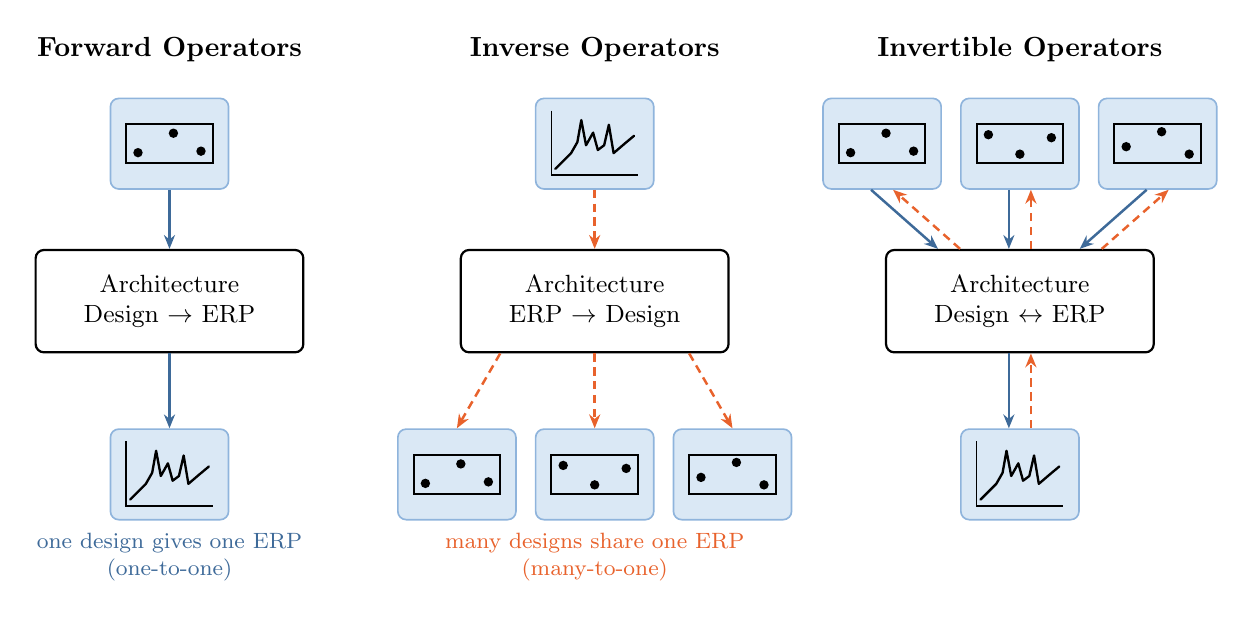
\begin{tikzpicture}
% ---- forward operators
\node[font=\bfseries] at (0,5.0) {Forward Operators};
\node[icon] (f1) at (0,3.8) {}; \plateicon{(f1.center)}{-0.8/-0.6, 0.1/0.7, 0.8/-0.5}
\node[plain, minimum width=3.4cm, minimum height=1.3cm] (fm) at (0,1.8) {Architecture\\ Design $\to$ ERP};
\node[icon] (f2) at (0,-0.4) {}; \spectrumicon{(f2.center)}
\draw[fwd] (f1.south) -- (fm.north);  \draw[fwd] (fm.south) -- (f2.north);
\node[note, text=fwdc] at (0,-1.45) {one design gives one ERP\\ (one-to-one)};
% ---- inverse operators
\node[font=\bfseries] at (5.4,5.0) {Inverse Operators};
\node[icon] (i1) at (5.4,3.8) {}; \spectrumicon{(i1.center)}
\node[plain, minimum width=3.4cm, minimum height=1.3cm] (im) at (5.4,1.8) {Architecture\\ ERP $\to$ Design};
\node[icon] (id1) at (3.65,-0.4) {}; \plateicon{(id1.center)}{-0.8/-0.6, 0.1/0.7, 0.8/-0.5}
\node[icon] (id2) at (5.4,-0.4)  {}; \plateicon{(id2.center)}{-0.8/0.6, 0/-0.7, 0.8/0.4}
\node[icon] (id3) at (7.15,-0.4) {}; \plateicon{(id3.center)}{-0.8/-0.2, 0.1/0.8, 0.8/-0.7}
\draw[inv] ($(im.south)+(-1.2,0)$) -- (id1.north);
\draw[inv] (im.south) -- (id2.north);
\draw[inv] ($(im.south)+(1.2,0)$) -- (id3.north);
\draw[inv] (i1.south) -- (im.north);
\node[note, text=invc] at (5.4,-1.45) {many designs share one ERP\\ (many-to-one)};
% ---- invertible operators
\node[font=\bfseries] at (10.8,5.0) {Invertible Operators};
\node[plain, minimum width=3.4cm, minimum height=1.3cm] (vm) at (10.8,1.8) {Architecture\\ Design $\leftrightarrow$ ERP};
\node[icon] (vd1) at (9.05,3.8)  {}; \plateicon{(vd1.center)}{-0.8/-0.6, 0.1/0.7, 0.8/-0.5}
\node[icon] (vd2) at (10.8,3.8)  {}; \plateicon{(vd2.center)}{-0.8/0.6, 0/-0.7, 0.8/0.4}
\node[icon] (vd3) at (12.55,3.8) {}; \plateicon{(vd3.center)}{-0.8/-0.2, 0.1/0.8, 0.8/-0.7}
\draw[fwd] ($(vd1.south)+(-0.14,0)$) -- ($(vm.north)+(-0.9-0.14,0)$);  \draw[inv] ($(vm.north)+(-0.9+0.14,0)$) -- ($(vd1.south)+(0.14,0)$);
\draw[fwd] ($(vd2.south)+(-0.14,0)$) -- ($(vm.north)+(-0.14,0)$);      \draw[inv] ($(vm.north)+(0.14,0)$) -- ($(vd2.south)+(0.14,0)$);
\draw[fwd] ($(vd3.south)+(-0.14,0)$) -- ($(vm.north)+(0.9-0.14,0)$);   \draw[inv] ($(vm.north)+(0.9+0.14,0)$) -- ($(vd3.south)+(0.14,0)$);
\node[icon] (v2) at (10.8,-0.4) {}; \spectrumicon{(v2.center)}
\draw[fwd] ($(vm.south)+(-0.14,0)$) -- ($(v2.north)+(-0.14,0)$);
\draw[inv] ($(v2.north)+(0.14,0)$) -- ($(vm.south)+(0.14,0)$);
\end{tikzpicture}
\end{document}
